\documentclass[12pt]{article}
\usepackage[usenames,dvipsnames,table]{xcolor}
\usepackage{graphicx,amsmath,amssymb,amsthm,multirow,array,bm,bbm,esint}
\usepackage{array,tikz-cd}
\usepackage{pgfplots}
\pgfplotsset{compat=1.15}
\usetikzlibrary{arrows}
\usetikzlibrary{backgrounds}
\usepackage{tikz}
\usetikzlibrary{decorations.markings}
\tikzset{middlearrow/.style={
        decoration={markings,
            mark= at position 0.5 with {\arrow{#1}} ,
        },
        postaction={decorate}
    }
}

\begin{document}

 	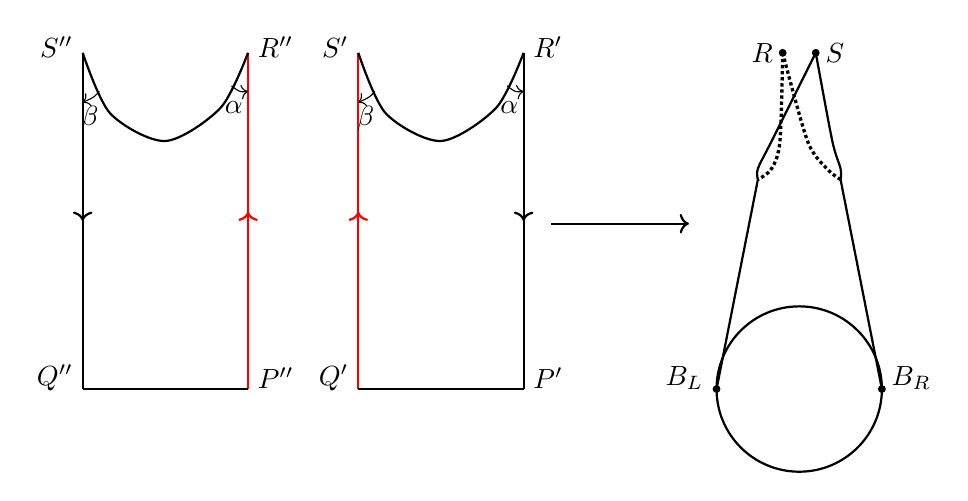
\begin{tikzpicture}[scale=.7]
	\draw[red,  thick,middlearrow={<}]plot [smooth] coordinates{(-10,6.1) (-10,0)};
	\draw[ middlearrow={>}, thick]plot [smooth] coordinates{(-13,6.1) (-13,0)};
	\draw[ thick]plot [smooth] coordinates{(-13,0) (-10,0)};
	\draw[red,  thick,middlearrow={<}]plot [smooth] coordinates{(-8,6.1) (-8,0)};
	\draw[ thick]plot [smooth] coordinates{(-13,6.1) (-12.5,5)(-11.5,4.5)(-10.5,5.1)(-10,6.1)};
	\draw[ thick]plot [smooth] coordinates{(-8,6.1) (-7.5,5)(-6.5,4.5)(-5.5,5.1)(-5,6.1)};
	\draw[  thick]plot [smooth] coordinates{(-8,0) (-5,0)};
	\draw[ middlearrow={>}, thick]plot [smooth] coordinates{(-5,6.1) (-5,0)};
	\draw[  thick,->]plot [smooth] coordinates{(-4.5,3) (-2,3)};
			\fill[draw=black, thick, fill=white!20] (0,0) circle[radius=1.5];
			\draw (-0.3,6.1)  node  [circle,fill,inner sep=1pt]{};
			\draw (0.3,6.1)  node  [circle,fill,inner sep=1pt]{};
			\draw (1.5,0) node  [circle,fill,inner sep=1pt]{};
			\draw (1.5,0.2) node [right]{$B_R$};
			\draw (-1.5,0) node  [circle,fill,inner sep=1pt]{};
			\draw (-2.6,0.2) node [right]{$B_L$};
			\draw (-0.3,6.1) node [left]{$R$};
			\draw (0.3,6.1) node [right]{$S$};
			\draw (-5,0.2) node [right]{$P'$};
			\draw (-5,6.2) node [right]{$R'$};
			\draw (-8,0.2) node [left]{$Q'$};
			\draw (-8,6.2) node [left]{$S'$};
			\draw (-10,0.2) node [right]{$P''$};
			\draw (-10,6.2) node [right]{$R''$};
			\draw (-13,0.2) node [left]{$Q''$};
			\draw (-13,6.2) node [left]{$S''$};
			\draw[->]plot [smooth] coordinates{(-5.3,5.5) (-5.15,5.4) (-5,5.4)};
			\draw (-5.6,5.1) node [right]{$\alpha$};
			\draw[<-]plot [smooth] coordinates{(-8,5.2) (-7.8,5.3) (-7.7,5.4)};
			\draw (-8.2,4.9) node [right]{$\beta$};
			\draw[->]plot [smooth] coordinates{(-10.3,5.5) (-10.15,5.4) (-10,5.4)};
			\draw (-10.6,5.1) node [right]{$\alpha$};
			\draw[<-]plot [smooth] coordinates{(-13,5.2) (-12.8,5.3) (-12.7,5.4)};
			\draw (-13.2,4.9) node [right]{$\beta$};
			%lower
			         %wormoholes 
         \draw [black, densely dotted, very thick]plot [smooth] coordinates {(-.3,6.1)(.15,4.5)(.5,4)(.75,3.8)} ;% inside curveR1
         \draw [black, thick]plot [smooth] coordinates {(0.3,6.1)(.6,4.5)(.75,4)(.75,3.8)} ;% inside curveR1
         \draw [black, densely dotted, very thick]plot [smooth] coordinates {(-.3,6.1)(-.35,4.5)(-.5,4)(-.75,3.8)} ;% inside curveR1
         \draw [black, thick]plot [smooth] coordinates {(0.3,6.1)(-.5,4.5)(-.75,4)(-.75,3.8)} ;% inside curveR1
                  \draw [black,thick]plot [smooth] coordinates {(.75,3.8)(1.5,0)} ;% bottom curveR
         \draw [black,thick]plot [smooth] coordinates {(-1.5,0)(-.75,3.8)} ;% bottom curveL
                         \end{tikzpicture}

\end{document}